\documentclass[journal,10pt,twocolumn]{article}
\usepackage{graphicx}
\usepackage[margin=0.5in]{geometry}
\usepackage{amsmath}
\usepackage{array}
\usepackage{booktabs}
\usepackage{listings}
\providecommand{\norm}[1]{\left\lVert#1\right\rVert}
\providecommand{\abs}[1]{\left\vert#1\right\vert}
\usepackage{enumerate}
\let\vec\mathbf
\newcommand{\myvec}[1]{\ensuremath{\begin{pmatrix}#1\end{pmatrix}}}
\newcommand{\mydet}[1]{\ensuremath{\begin{vmatrix}#1\end{vmatrix}}}
\providecommand{\brak}[1]{\ensuremath{\left(#1\right)}}
\lstset{
frame=single,
breaklines=true,
columns=fullflexible
}
\title{\textbf{Matrix Assignment}}
\author{ALURU AJAY}
\date{September 2022}
\begin{document}
\maketitle

\section{Problem Statement}
In a triangle ABC, E is the mid-point of median AD.
\vspace{0.3cm}\\ 
Show that ar($\Delta BED$) = $\frac{1}{4}$ ar($\Delta ABC$)

\section{Diagram}
Plot of Triangle is shown in figure 1, where point B is origin and points A, B, C and D are the vertices of Triangle.
\begin{figure}[h]
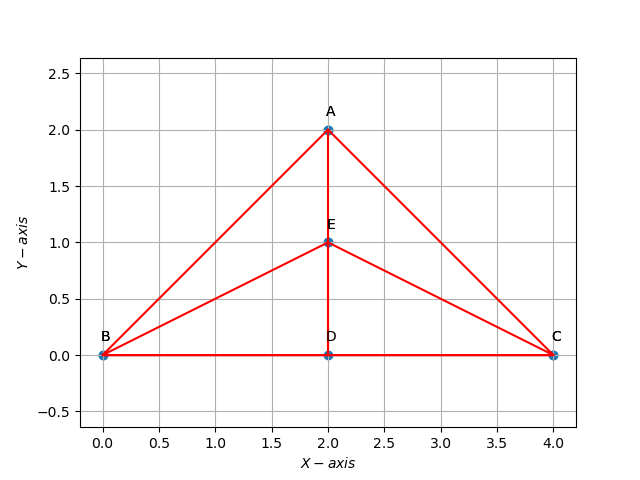
\includegraphics[scale=0.6]{fig_Triangle.png}
\caption{Triangle}
\label{fig:Triangle}
\end{figure}

\section{PROOF}
In $\Delta ABC$,with AD as median
E is the mid-point of AD
\begin{center}
    $||{\vec{E-A}}||$ = $||{\vec{E-D}}||$
\end{center}
\begin{center}
\begin{equation}
    ||{\vec{D-B}}|| = \frac{1}{2} ||{\vec{C-B}}||
\end{equation}
\end{center}
\begin{flushleft}
From $\Delta ABC$
\end{flushleft}
\begin{equation}
    ar(\Delta ABC) = \frac{1}{2} \times ||{\vec{B-A}}|| \times ||{\vec{C-B}}||
\end{equation}
\begin{flushleft}
From $\Delta BED$
\vspace{0.3cm}\\
ar($\Delta BED$) = $\frac{1}{2}$ $\times$ $||{\vec{E-B}}||$ $\times$ $||{\vec{D-B}}||$
\vspace{0.3cm}\\
From Eq(1) we can write as
\begin{equation}
    ar(\Delta BED) = \frac{1}{2} \times ||{\vec{E-B}}|| \times\frac{1}{2} ||{\vec{C-B}}||
\end{equation}
We know that from Parallelogram law of Vector Addition
\begin{equation}
     \vec{E-B} = \frac{1}{2} ((\vec{B-A}) + \vec{C-B}))
\end{equation}
Substituting Eq(4) in Eq(3) $\And$ re-writing the Eq(3)\\
\vspace{0.3cm}
ar($\Delta BED$) = $\frac{1}{2}$ $\times$ (($\frac{1}{2}$$||{\vec{(B-A) + (C-B)}}||$) $\times$$\frac{1}{2}$ $||{\vec{C-B}}||$)
\vspace{0.5cm}\\
ar($\Delta BED$) = $\frac{1}{2}$ $\times$ $\frac{1}{4}$($||{\vec{B-A}}||$ $\times$ $||{\vec{C-B}}||$)
\vspace{0.5cm}\\
ar($\Delta BED$) =$\frac{1}{4}$ ($\frac{1}{2}$ $\times$ $||{\vec{B-A}}||$ $\times$ $||{\vec{C-B}}||$)
\vspace{0.5cm}\\
From Eq(2)
\vspace{0.3cm}\\
ar($\Delta BED$) =$\frac{1}{4}$(ar($\Delta ABC$)
\end{flushleft}
\vspace{0.5cm}
\centering
\begin{tabular}{|c|}
\hline
Ar($\Delta$ BED) = $\frac{1}{4}$ Ar($\Delta$ ABC)\\
\hline
\end{tabular}\\
\vspace{0.5cm}
Hence Proved

\begin{flushleft}
\section{Software}
\end{flushleft}
Download the codes given in the link below and execute them.\\
\begin{table}[h]
\centering
\begin{tabular}{|c|} \hline
\rule{0pt}{10pt} 
https://raw.githubusercontent.com/19PA1AO410/\\
FWC-Module-1/main/Matrix%20_Assignment/line_assignment/line.py
\\\hline
 \end{tabular}
\end{table}
\bibliographystyle{ieeetr}
\end{document}
\end{document}
